% VERWENDET !!
Web-Anwendungen sind ein fester Bestandteil, wenn es um online Service geht. Im selben Zuge werden immer mehr Anfälligkeiten in solchen entdeckt und offengelgt. \autocite[1]{kirda2009}

% VERWENDET !!
\textcite[4]{flanagan2017} erklärt, dass JavaScript eine interpretierte Programmiersprache mit Objectorientierte Möglichkeiten. Sie wird heutzutage großteils dazu genutzt um die client-seitige Darstellung von Webseiten zu verbessern.
JavaScript lauft seit dem Jahr 1997 unter dem Standard ECMAScript\cite[43]{ecma2018} läuft, ist eine Spezifikation davon. Wenn nun ein Web-Browser mit einem JavaScript Interpreter erweitert ist, ermöglicht dieser die Verteilung von ausführbaren Inhalten mittels script.

% VERWENDET !!
Nach \textcite[1]{kirda2009} kann vom Interpreter automatisch ausgeführter JavaScript Code einen möglichen Raum für Angriffe gegen die Benutzerumgebung darstellen. Eine sichere Ausführung von JavaScript Code basiert auf dem Prinzip einer Sandbox\footnote[1]{https://de.wikipedia.org/wiki/Sandbox}. Diese erlaubt es dem Code nur gewisse Operationen auszuführen und gewährt nur begrenzten Zugriff auf Ressourcen im Web-Browser. Ebenso werden JavaScript Programme von verschiedenen Seiten mit einem Abschottungsmechanismus, der "same origin policy"\footnote[2]{https://de.wikipedia.org/wiki/Same-Origin-Policy} geschützt. Diese erlaubt es dem Programm nur auf Ressourcen innerhalb seines Ursprungs zuzugreifen.

% VERWENDET !!
In der heutigen Zeit nutzen die meisten Webseiten die Funktionalität von JavaScript im Web-Browser als deren großen Vorteil, doch trotz Einhaltung der "same origin policy" kann immer noch die Sicherheit des Systems verletzt werden. Dies geschieht, wenn beispielsweise ein Nutzer dazu gebracht wird, sich schadhaften JavaScript Code, welcher zuvor von einem Angreifer erstellt worden ist, herunterzuladen. Diese im wahrsten Sinne des Wortes technische Ausbeutung nennt man eine "cross-site scripting"(XSS) Attake.\autocite[2]{kirda2009}

% VERWENDET !!
\begin{figure}[ht]
	\centering
	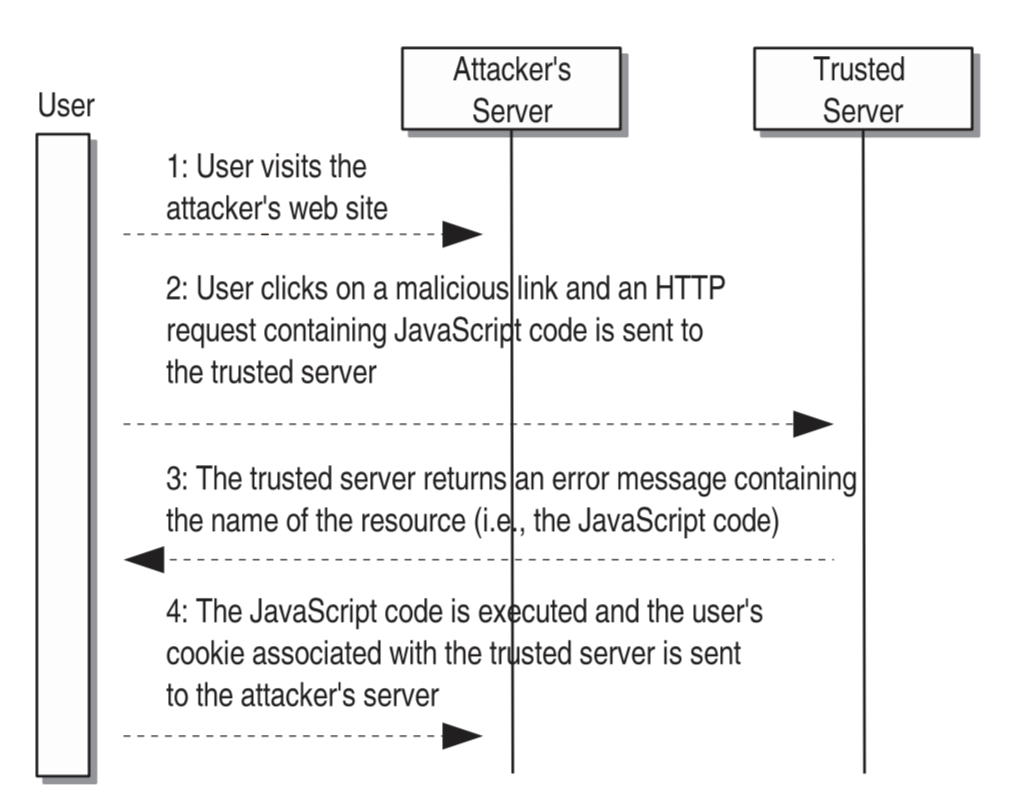
\includegraphics[width=0.5\linewidth]{images/cross-site-scripting_scenario-kirda2009_p2.png}
	\caption{Fig.1 - Ein typischen cross-site scripting Szenarium\autocite[p]{kirda2009}}
\end{figure}
